
\section*{Zielsetzung}
Das Ziel dieses Projektes ist es einen Regelkreis für eine sich selbst regulierende, indoor hydroponics Pflanzenzucht zu bauen.
Es soll die Düngekonzentration im Wasser, sowie der pH-Wert der Lösung durch geregelte Dünger und pH-Buffer Zugabe gesteuert werden.

\section*{Projektaufbau}
Um das Problem der Düngekonzentration in einem für uns umsetzbaren Rahmen zu halten, wird die relative Ionenkonzentration untereinander, während eines Wachstumszyklus, vorersts als konstant angenommen.
Die Düngekonzentration kann somit als direkt proportional zur elektrischen Leitfähigkeit (EC) der Flüssigkeit modelliert werden.
Fällt einer der Ist-Werte unter den Soll-Zustand, so wird mittels dem selbstgebaute rotary-vane-pump gegengesteuert (Dünger oder pH-UP/-Down).
Aus den Temperatur-, EC- und pH-Wert-Daten soll dann ebenso ein Modell für die Löslichkeit der Düngesalze, bzw. die zeitabhängige Veränderung des EC-Wertes bei Zugabe des Düngers, erstellt werden.

\begin{figure}[H]
    \centering
    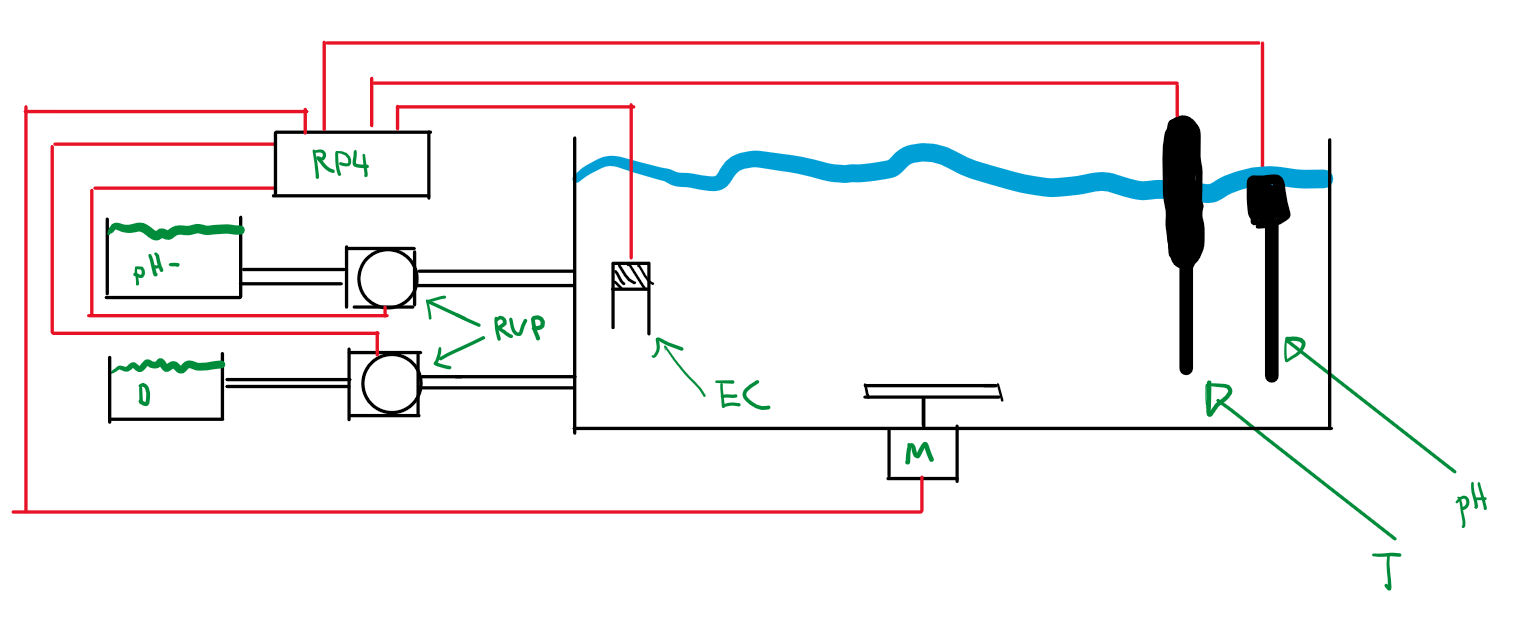
\includegraphics[width=\linewidth]{skizze.png}
    \caption{
        Skizze des Regulierungsaufbaus am Wasserreservoir.
        \textbf{pH-}: (pH-)-Lösung; 
        \textbf{D}: Dünger-Lösung; 
        \textbf{RVP}: Rotary-Vane-Pump; 
        \textbf{EC}: Leitfähigkeitssensor; 
        \textbf{M}: Rührmotor; 
        \textbf{RP4}: Raspberry Pi 4; 
        \textbf{T}: Thermometer; 
        \textbf{pH}: ph-Messgerät;
    }
\end{figure}

\section*{Physikalische Anforderungen}
\begin{enumerate}
    \item Ausreichende Genauigkeit der Rotary-Vane-Pumps für gute Regelantwort.
    \item Konsistente Messgenauigkeit des pH- und EC-Sensors.
    \item Entwicklung eines Löslichkeitsmodells
\end{enumerate}


\section*{Komponenten und Kosten}
\begin{table}[H]
    \centering
    \caption{
        Skizze
    }
    \begin{tabular}{| c | c |}
        \hline
        Komponente &  Kosten / \euro{}\\
        \hline
        EC-Sensor & 15 - 70  \\
        \hline
        pH-Sensor & 30 - 70  \\
        \hline
        Temperatur-Sensor & 5 - 20  \\
        \hline
        Rührmotor & 5 - 10  \\
        \hline
        Rotary-Vane-Pumps & 30 - 50  \\
        \hline
        Raspberry Pi & vorhanden  \\
        \hline
        sonstiger Aufbau & 20 - 40  \\
        \hline
        \hline
        Summe & 105 - 260  \\
        \hline
    \end{tabular}
    \label{tab:Komponenten}
\end{table}


\section*{Software}
\begin{enumerate}
    \item Sensormessungen und Motorsteuerung (Python oder C)
    \item Regelungsmodell (Python)
\end{enumerate}

\section*{Aufwandsabschätzung}
\begin{table}[H]
    \centering
    \caption{
        Skizze
    }
    \begin{tabular}{| c | c |}
        \hline
        Arbeitspaket &  Aufwand / h\\
        \hline
        Sensormessung und Motorsteuerung & 20 - 40  \\
        \hline
        Regelungsmodell & 30 - 50  \\
        \hline
        Rotary-Vane-Pumpen & 5 - 15  \\
        \hline
        Mechanischer Aufbau & 10 - 20  \\
        \hline
        Sensor-/Aktor-Kalibrierung & 30 - 50  \\
        \hline
        Debugging & 40 \\
        \hline
        \hline
        Summe & 135 - 205  \\
        \hline
    \end{tabular}
    \label{tab:Aufwand}
\end{table}
\section*{Bonus-Task:}
Ursprünglich wollten wir die Konzentration der einzelnen, gelösten Ionen bestimmen.
Da diese Form der Analyse aber zum einen sehr aufwendig, und schlimmer noch, extrem kostenintensiv ist, scheint Spektroskopie im IR-Bereich für unsere Zwecke am hilfreichsten zu sein(Das Verhältnis der Hauptkomponenten unseres Düngers lässt sich durch IR-Spektroskopie abschätzen). Da der zusätzliche Bau eines Spektroskops zu viel für den Rahmen dieses Projektes wäre, könnten wir, falls möglich, einen komerziellen Spektrographen zu Vorführungszwecken benutzen und die Daten in unsere Modellierung mit ein beziehen. Dies wäre allerdings nur als Bonus zum Projekt gedacht und gehört nicht zum eigentlichen Projektvorschlag.
